\documentclass{beamer}

% Beamer style
%\usetheme[secheader]{Madrid}
\usetheme{CambridgeUS}
\usecolortheme[rgb={0.65,0.15,0.25}]{structure}
%\usefonttheme[onlymath]{serif}
\beamertemplatenavigationsymbolsempty
%\AtBeginSubsection

% Packages
%\usepackage[french]{babel}
\usepackage[latin1]{inputenc}
\usepackage{color}
\usepackage{dsfont, stmaryrd}
\usepackage{amsmath, amsfonts, amssymb}
\usepackage{epsfig}
\usepackage{/Latex/astats}
%\usepackage[all]{xy}
\usepackage{graphicx}

% Commands
\definecolor{darkred}{rgb}{0.65,0.15,0.25}
\newcommand{\emphase}[1]{\textcolor{darkred}{#1}}
\newcommand{\paragraph}[1]{\noindent\emphase{#1}}
\newcommand{\refer}[1]{\textcolor{blue}{\sl \cite{#1}}}
\newcommand{\referSR}[2]{\textcolor{blue}{\sl \nocite{#1}#2}}
\newcommand{\ra}{$\rightarrow$~}
\newcommand{\newblock}{}

% Symbols
\newcommand{\BIC}{\text{BIC}}
\newcommand{\Bias}{\mathbb{B}}
\newcommand{\dd}{\text{d}}
\newcommand{\Esp}{\mathbb{E}}
\newcommand{\Ebf}{{\bf E}}
\newcommand{\Ecal}{\mathcal{E}}
\newcommand{\ICL}{\text{ICL}}
\newcommand{\Ibb}{\mathbb{I}}
\newcommand{\Cov}{\mathbb{C}\text{ov}}
\newcommand{\Var}{\mathbb{V}}
\newcommand{\pen}{\text{pen}}
\newcommand{\Hbf}{{\bf H}}
\newcommand{\Hcal}{\text{H}}
\newcommand{\Lcal}{\mathcal{L}}
\newcommand{\Mcal}{\mathcal{M}}
\newcommand{\Ncal}{\mathcal{N}}
\newcommand{\Ocal}{\mathcal{O}}
\newcommand{\Pbf}{{\bf P}}
\newcommand{\Pcal}{\mathcal{P}}
\newcommand{\Scal}{\mathcal{S}}
\newcommand{\Ucal}{\mathcal{U}}
\newcommand{\Vcal}{\mathcal{V}}
\newcommand{\Tbf}{{\bf T}}
\newcommand{\Ubf}{{\bf U}}
\newcommand{\Ybf}{{\bf Y}}
\newcommand{\Zbf}{{\bf Z}}
\newcommand{\Pibf}{\mbox{\mathversion{bold}{$\Pi$}}}
\newcommand{\mubf}{\mbox{\mathversion{bold}{$\mu$}}}
\newcommand{\thetabf}{\mbox{\mathversion{bold}{$\theta$}}}


%====================================================================
\title[]{Statistical analysis of bio-molecular data and combinatorial
  difficulties: 2 examples}

\author{S. Robin}

\institute[AgroParisTech / INRA]{AgroParisTech / INRA \\
  \bigskip
  \begin{tabular}{ccccc}
    
\epsfig{file=/Latex/Logo/LogoINRA-Couleur.ps, width=2.5cm} &
    \hspace{.5cm} &
    
\epsfig{file=/Latex/Logo/logagroptechsolo.eps, width=3.75cm} &
    \hspace{.5cm} &
    \epsfig{file=/Latex/Logo/Logo-SSB.eps, width=2.5cm} \\
  \end{tabular} \\
  \bigskip
  }

\date[January'10]{Challenging problems in Statistical Learning,\\ Paris
  I, January 2010}
%====================================================================

%====================================================================
%====================================================================
\begin{document}
%====================================================================
%====================================================================

%====================================================================
\frame{\titlepage}
%====================================================================

%====================================================================
%====================================================================
\section{Introduction}
\frame{ \frametitle{Introduction} 
%====================================================================
  \paragraph{General purpose}
  \begin{itemize}
  \item Statistical inference often faces combinatorial issues 
  \item that may lead to prohibitive computational burden, especially
    for high-dimensional data 
  \item but that can be circumvented at the price of some algebraic
    manipulations.
  \end{itemize}

  \bigskip
  \paragraph{2 examples from bio-molecular data analysis}
  \begin{enumerate}
  \item Multiple testing \& Histogram selection: \emphase{A. Celisse}
  \item Chromosomal aberrations \& Breakpoint detection:
    \emphase{G. Rigaill \& E. Lebarbier}
  \end{enumerate}
  }

% %====================================================================
% \frame{ \frametitle{Outline}
% %====================================================================
  
%   \tableofcontents
% %  \tableofcontents[pausesections]
%   }

%====================================================================
%====================================================================
\section{Histogram selection}
\subsection{Density estimation}
\frame{ \frametitle{Density estimation} \pause
%====================================================================
  \paragraph{An old problem:} Estimate $g$ based on
  $\{X_1, \dots, X_m\}$ i.i.d., $X_j \sim g$.

  \bigskip
  \paragraph{Kernel estimate:} For a kernel $K_h$, with bandwidth $h$:
  $$
  \widehat{s}(x) = \frac1{mh} \sum_j K_h(x - X_j).
  $$

  \bigskip
  \paragraph{Histogram estimate:} For a partition of $[0, 1]$ in $D$
  bins $I = \{I_k\}, k=1,...,D$ (with length $w_k = |I_k|$):
  $$
   \widehat{s}(x) = \sum_k \frac{m_k}{m w_k} \Ibb\{x \in I_k\},
  $$
  where $m_k = \sum_j \Ibb\{X_j \in I_k\}$.  
  }

%====================================================================
\frame{ \frametitle{Quadratic loss}
%====================================================================
  \paragraph{$\ell_2$ loss:} The best possible estimate $s$ of a true
  density $g$ within a collection $\Scal$ can be defined as
%   \begin{eqnarray*}
%     \widetilde{s} & = & \arg\min_{s \in \Scal} \Esp_g[\|s - g\|^2] \\
%     & = & \arg\min_{s \in \Scal} \Esp_g[\|s\|^2]  - 2 \int s(x)g(x)\dd
%     x \\
%     & = & \arg\min_{s \in \Scal} R(s)
%   \end{eqnarray*}
  $$
    \widetilde{s} = \arg\min_{s \in \Scal} \Esp_g[\|s - g\|^2] 
    = \arg\min_{s \in \Scal} \underset{R(s)}{\underbrace{
        \left(\Esp_g[\|s\|^2]  - 2 \int s(x)g(x)\dd x \right) }}
  $$

  \bigskip
  \paragraph{Leave $p$ out (LpO) estimation of $R({s})$:}
  $$
  \widehat{R}_p({s}) = \binom{m}{p}^{-1} \sum_{e \in \Ecal_p}
  \left[\|{s}^{\overline{e}}\|^2 - \frac2p \sum_{j \in e}
    {s}^{\overline{e}}(x_j) \right]
  $$
  where $\Ecal_p$ is the set of all subsets of $\{1, \dots, m\}$ of
  size $p$ and 
  $$
  \overline{e} = \{1, \dots, m\} \setminus e.
  $$
  }

%====================================================================
\subsection{Cross-validation}
\frame{ \frametitle{Explicit formulas}
%====================================================================
  \paragraph{LpO in practice:}
  \begin{itemize}
  \item The exploration of all the $\binom{m}{p}$ subsets is generally
    out of reach. 
  \item LpO is often replaced by V-fold (with $V = p/m$) where only
    $V$ (random disjoint) subsets are considered
  \end{itemize}

  \bigskip \pause
  \paragraph{Specific case of histograms:} based on some combinatorial
  manipulations 
  $$
  \widehat{R}_p(s_w) = \frac{2m - p}{(m - 1)(m - p)} \sum_k
  \frac{m_k}{m w_k} - \frac{m(m - p + 1)}{(m - 1)(m - p)} \sum_k
  \frac1{w_k} \left(\frac{m_k}m\right)^2
  $$
  \referSR{CeR08}{Celisse \& R. (08)}

  \bigskip
  A similar formula can be derived for \emphase{kernel density estimates} .
  }

%====================================================================
\frame{ \frametitle{Moments of the LpO estimate}
%====================================================================
  Denoting $\alpha_k = \Pr\{X \in I_k\}$, additional cobinatorial
  manupilations lead to 
  \begin{eqnarray*}
     {\Bias}[\widehat{R}_p(s_w)] & = & \frac{p}{m(m-p)} \sum_k
     \frac{{\alpha}_k(1-{\alpha}_k)}{w_k} \\
    {\Var}[\widehat{R}_p(s_w)] & = & \frac{p^2 \phi_2(n,
    {\alpha}, w) + p \phi_1(n, {\alpha}, w) +
    \phi_0(n, {\alpha}, w)}{[n(n - 1)(n - p)]^2}
  \end{eqnarray*}
  
  \bigskip
  \paragraph{Plug-in estimates:}
  \begin{itemize}
  \item Estimates of ${\Bias}[\widehat{R}_p(s_w)]$ and
    ${\Var}[\widehat{R}_p(s_w)]$ can be obtained with
    $$
    \widehat{\alpha}_k = m_k/m.
    $$
  \item Their accuracy can be controled via Bernstein inequality.
  \end{itemize}
  }

%====================================================================
\frame{ \frametitle{Comparison with V-fold}
%====================================================================
  \vspace{-1cm}
  $$
  \hspace{-.4cm}
  \begin{tabular}{ll}
    \begin{tabular}{p{6cm}}
      Both $\widehat{R}_{\text{LpO}}$ and
      $\widehat{R}_{\text{V-fold}}$ are unbiased 
      $$
      \Esp[\widehat{R}_{\text{LpO}}(s)] =
      \Esp[\widehat{R}_{\text{V-fold}}(s)] = R(s)
      $$
      but due to the additional randomness in the choice of the $V$
      subsets, 
      $$
      \Var[\widehat{R}_{\text{LpO}}(s)] <
      \Var[\widehat{R}_{\text{V-fold}}(s)].
      $$
      \paragraph{Right panel:} \\
      $m = 500, p = 100, V = 5$.
    \end{tabular}
    &
    \begin{tabular}{p{6cm}}
      \paragraph{Choice of $h$ for a kernel} \\
      \\
      \includegraphics[width=5cm, bbllx=142, bblly=424, bburx=399,
      bbury=663, clip=]{../Figures/CeR08-CSDA-Fig1} 
    \end{tabular}
  \end{tabular}
  $$
  $
  \text{--}: \widehat{R}_{\text{LpO}}(s), \quad
  \textcolor{red}{\text{- -}}: + 2
  \sqrt{\widehat{\Var}[\widehat{R}_{\text{V-fold}}(s)]}, \qquad 
  \textcolor{blue}{\cdots}: - 2
  \sqrt{\widehat{\Var}[\widehat{R}_{\text{V-fold}}(s)]}
  $
%       $\begin{array}{ll}
%         \text{--} & \widehat{R}_{\text{LpO}}(s) \\
%         \textcolor{red}{\text{- -}} & + 2
%         \sqrt{\widehat{\Var}[\widehat{R}_{\text{V-fold}}(s)]} \\
%         \textcolor{blue}{\cdots} & + 2
%         \sqrt{\widehat{\Var}[\widehat{R}_{\text{V-fold}}(s)]}
%       \end{array}$

  }

%====================================================================
\frame{ \frametitle{Choice of $p$}
%====================================================================
  \paragraph{The best' $p$} can be chosen adaptively so that
  $\widehat{R}_p(s_w)$ provides the best estimate of ${R}(s_w)$. We'd
  like a small
  $$
  MSE(\widehat{R}_p(s_w)) = \Esp[\widehat{R}_p(s_w) - {R}(s_w)]^2.
  $$

  \bigskip
  \paragraph{Selection procedure:}
  \begin{itemize}
  \item Based on the \emphase{plug-in estimates}, the explicit
    formulas allow to \emphase{choose $p$ adaptively}, e.g.
    $$
    \widehat{p} = \arg\min_p \;
    \widehat{\text{MSE}}[\widehat{R}_p(s_w)] = \arg\min_p \;
    \widehat{\Bias}^2[\widehat{R}_p(s_w)] +
    \widehat{\Var}[\widehat{R}_p(s_w)].
    $$
  \item For bandwidth selection in both kernel and regular histograms,
    $\widehat{p}$ is often 1. \\
    \ra \emphase{Leave-one-out} performs well.
  \end{itemize}
  }

%====================================================================
\section{Multiple testing} 
\subsection{Differential analysis}
\frame{ \frametitle{Application to gene expression data} \pause
%====================================================================
  \paragraph{'High throughput' technologies:} Microarrays, SAGE, Next
  generation sequencing (NGS) \\
  \ra monitoring of the expression level of all genes of a
  given species \\
  \ra $m = 10^3 - 10^4$ expression measures per experiments \\

  \bigskip 
  \paragraph{Differential analysis:} Detection of the genes associated
  with a given biological process (response to a stress, cancer
  development, etc.) \\
  \ra for each gene $j$ ($j=1..m$), we need to test
  $$
  \Hbf_{0, j} = \{\text{gene $j$ has the same expression level in
    conditions $A$ and $B$}\}
  $$

  \bigskip 
  \paragraph{Multiple testing:} Large number of tests \\
  \ra Need to control for multiple testing to avoid numerous false
  positives }

%====================================================================
\frame{ \frametitle{Multiple testing procedures}
%====================================================================
  \paragraph{Family-Wise Error Rate (FWER) =} 
  $ \Pr\{\text{Number of rejected true $\Hbf_{0, j}$} > 0\} $ \\
  \ra To ensure $FWER \leq \alpha$:
  $$
    \text{Reject $\Hbf_{0, j}$ if } \left\{
        \begin{tabular}{ll}
          $P_j \leq  1 - (1-\alpha)^{\emphase{m_0}}$ & (Sidak:
          independent test) \\ 
          $P_j \leq  \alpha / \emphase{m_0}$ & (Bonferroni) \\
        \end{tabular}
      \right.
  $$

  \bigskip 
  \paragraph{False Discovery Rate (FDR) =}
  $
  \displaystyle{
    \Esp\left[\frac{\text{\# rejected true $\Hbf_{0, j}$}}{\text{\#
  rejected $\Hbf_{0, j}$}}\right] }
  $
  \ra Benjamini-Hochberg procedure for ordered $p$-values $P_{(j)}$:
  $$
  \text{Reject $\Hbf_{0, j}$ if } P_{(j)} \leq \alpha \; j /
  \emphase{m_0}
  \qquad \Rightarrow \qquad
  FDR \leq \alpha
  $$

  \bigskip 
  \paragraph{Conservative strategy:} Replace $m_0 = $ \# true null
  hypotheses $\Hbf_{0, j}$ with $m$.
  }

%====================================================================
%====================================================================
\subsection{Estimation of $m_0$}
\frame{ \frametitle{Estimating $m_0$}
%====================================================================
  A good estimate of $m_0$ (or of $\pi_0 = m_0/m$) would
  \emphase{improve the power} of the multiple test procedure.  
  $$
  \hspace{-.4cm}
  \begin{tabular}{ll}
    \begin{tabular}{p{6cm}}
      \paragraph{Distribution of $P$:}
      $$
      \begin{array}{lrcl}
        \text{under } \Hbf_0 & P & \sim & \Ucal_{[0,1]} \\
        \text{under } \Hbf_1 & P & \sim & F \\
      \end{array}
      $$
      with $\Esp(F)$ '\emphase{small}'.
      
      \bigskip 
      \refer{Sto01}: for a 'sufficiently' large threshold
      $\lambda^*$,
      $$
      \widehat{\pi}_0(\lambda^*)  = \frac{\#\{j: p_j > \lambda^*\}}{m
        (1-\lambda^*) }
      $$
    \end{tabular}
    &
    \begin{tabular}{c}
      \includegraphics[width=5cm]{../Figures/FigStorey}
    \end{tabular}
  \end{tabular}
  $$
  \bigskip
  \paragraph{Our goal:} Chose $\lambda^*$ based on a sample of
  $p$-values $(P_1, \dots, P_m)$.
  }

%====================================================================
\frame{ \frametitle{Histogram density estimate}
%====================================================================
  The choice of $\lambda$ can be rephrased in terms of
  choice of an histogram with \emphase{irregular bins}.
  $$
  \hspace{-.4cm}
  \begin{tabular}{ll}
    \begin{tabular}{p{6cm}}
      \paragraph{Histogram collection $\Mcal$:}
      \begin{itemize}
      \item Based on a regular grid with $D$ bins ($D = D_{\min} \dots
        D_{\max}$); %: $w_k = 1/D$
      \item Merge all \emphase{bins on the right} from $\lambda = d/D$
        to 1 ($d = 0 \dots D$);
      \item \emphase{$|\Mcal| = \Ocal(D^2_{\max})$}
      \end{itemize}

      $$
      \emphase{\widehat{\lambda}} = \lambda\left(
      \arg\min_{s  \in \Mcal}\widehat{R}_{\widehat{p}}(s) \right).
      $$
    \end{tabular}
    &
    \begin{tabular}{c}
      \includegraphics[width=5cm]{../Figures/FigCelisse}
    \end{tabular}
  \end{tabular}
  $$
  \begin{itemize}
  \item \paragraph{$\pi_0$ estimate} $\propto$ probability associated
    with the \emphase{largest bin}.  
  \item The \emphase{consistency} of $\widehat{\pi}_0$ can also be
    proved.
  \end{itemize}
  }

%====================================================================
\frame{ \frametitle{Case of a U-shaped density}
%====================================================================
  U-shaped distribution of the $p$-value may be encountered when
  considering one-sided tests.
  $$
  \hspace{-.4cm}
  \begin{tabular}{ll}
    \begin{tabular}{p{6cm}}
      \paragraph{Histogram collection $\Mcal'$:}
      \begin{itemize}
      \item Based on a regular grid with $D$ bins ($D = D_{\min} \dots
        D_{\max}$); 
      \item Merge all \emphase{central bins} from $\lambda = d/D$ to
        $\mu = d'/D$ ($1 \leq d < d' \leq D$);
      \item \emphase{$|\Mcal'| = \Ocal(D^3_{\max})$}
      \end{itemize}

      $$
      \emphase{[\widehat{\lambda}, \widehat{\mu}]} = [\lambda, \mu]\left(
      \arg\min_{s \in \Mcal'} \widehat{R}_{\widehat{p}}(s) \right).
      $$
    \end{tabular}
    &
    \begin{tabular}{c}
      \includegraphics[width=5cm]{../Figures/FigCelisse2}
    \end{tabular}
  \end{tabular}
  $$
  }

%======================================\==============================
\frame{ \frametitle{Simulations}
%====================================================================
  LpO provides more precise estimates than LOO.
  $$
  \includegraphics[width=11cm, height=6.25cm, clip=]{../Figures/CeR10-JSPI-Tab3} 
  $$
  The both outperforms other competing methods.
  }

%====================================================================
\section{Detection of genomic alterations}
\subsection{Genomic alterations}
\frame{ \frametitle{Genomic alterations in cancer cells} \pause
%==================================================================== 
  Genomic alterations are associated with (responsible for?) various
  types of cancers.
  $$
  \begin{tabular}{cc}
    Normal cell & Tumour cell \\
    \epsfig{file =
    /Recherche/Ruptures/Exposes/Figures/KaryotypeCancer-PH.ps, clip=,
    bbllx=325, bblly=676, bburx=468, bbury=780, scale=.9} 
  
    &
      \epsfig{file =
    /Recherche/Ruptures/Exposes/Figures/KaryotypeCancer-PH.ps, clip=,
    bbllx=127, bblly=676, bburx=319, bbury=780, scale=.9} 
    \end{tabular}
  $$
  \refer{Hup08} %\refer{Hup�}{08}
  }

%====================================================================
\subsection{CGH technology}
\frame{ \frametitle{CGH array technology}
%==================================================================== 
  Comparative Genomic Hybridisation = hybridisation of 2 DNA samples
  (\textcolor{red}{test} / \textcolor{green}{reference}) on a same
  chip. 
  $$
  \epsfig{file = /Recherche/Ruptures/Exposes/Figures/principe_CGH.eps, clip=,
    bbllx=0, bblly=61, bburx=700, bbury=478, scale=0.4}
  $$
  \refer{Pic05}
  }

%====================================================================
\frame{ \frametitle{A segmentation problem}
%==================================================================== 
  \begin{tabular}{ccccc}
    \multicolumn{3}{c}{Zoom on CGH profile} & \quad & Karyotype \\
    chrom. 1 & \quad & chrom. 17 \\
                                %   \epsfig{file = /Recherche/Ruptures/Exposes/Figures/Karyotype-CGH-PH.ps, clip=,
                                %     bbllx=80, bblly=617, bburx=150, bbury=763, scale=2}
    \epsfig{file = /Recherche/Ruptures/Exposes/Figures/Karyotype-CGH-PH.ps, clip=,
      bbllx=80, bblly=617, bburx=150, bbury=700, scale=1.5}
    & &
                                %   \epsfig{file = /Recherche/Ruptures/Exposes/Figures/Karyotype-CGH-PH.ps, clip=,
                                %     bbllx=270, bblly=617, bburx=300, bbury=763, scale=2}
    \epsfig{file = /Recherche/Ruptures/Exposes/Figures/Karyotype-CGH-PH.ps, clip=,
      bbllx=270, bblly=617, bburx=300, bbury=700, scale=1.5}
    & &
    \epsfig{file = /Recherche/Ruptures/Exposes/Figures/Karyotype-CGH-PH.ps, clip=,
      bbllx=364, bblly=617, bburx=485, bbury=763, scale=1}
  \end{tabular}

  \refer{Hup08}
  }

%====================================================================
\subsection{Change-point model}
\frame{ \frametitle{Change-point model} \pause
%==================================================================== 
  \emphase{Notations:}
  \begin{itemize}
  \item $K = $ number of segments
  \item $r = $ region $\llbracket \tau_r, \tau^r \rrbracket$; $n_r =$
    length of $r$
  \item $m = $ segmentation: $m = \{r_1, \dots, r_K: \tau_{r+1} =
    \tau^r +1\}$
  \item $Y_t = $ signal at position $t$ ($t \in \llbracket 1, n
    \rrbracket$); $\Ybf = \{Y_t\}$.
  \end{itemize}
  \bigskip
  \emphase{Model:}
  \begin{itemize}
  \item $\{Y_t\}$ independent
  \item $t \in r$: 
    $$
    Y_t \sim p(\cdot | \theta_r)
    $$
  e.g. 
  $$
  p(\cdot|\theta_r) = \Ncal(\mu_r, \sigma^2), \qquad \Ncal(\mu_r,
  \sigma^2_r), \qquad \Pcal(\lambda_r)
  $$
  \end{itemize}
  \refer{PRL05}
  }

%====================================================================
\frame{ \frametitle{Optimal segmentation}
%==================================================================== 
  For a given dimension $K$, the maximum likelihood estimate (MLE) is
  $$
  (\widehat{m}(K), \widehat{\thetabf}(m)) = \underset{m \in
    \Mcal_K, \thetabf}{\arg\max} \; p(\Ybf | m, \thetabf)
  $$
  where $\Mcal_K$ is the set of all segmentations with dimension $K$:
  $$
  |\Mcal_K| = \binom{n-1}{K-1}
  $$ 
  \begin{itemize}
  \item \emphase{Exhaustive search} among $\Mcal_K$ can not be
    achieved.
  \item \emphase{Dynamic programming} provides maximum likelihood
    $(\widehat{m}, \widehat{\thetabf})$ with complexity $\Ocal(n^2)$.
%     in both homoscedastic and heteroscedastic cases.
  \item Due to the \emphase{discontinuity of $p(\Ybf|m, \thetabf)$
      with respect to $m$}, standard maximum likelihood theory
    \emphase{does not apply to $\widehat{m}$}.  \\
    \ra Inference (e.g.  confidence interval) of the breakpoints is
    not standard.
  \end{itemize}
  }

%====================================================================
\section{Distribution over the segmentation space}
\subsection{Exploration the segmentation space}
\frame{ \frametitle{Dynamic programming} \pause
%==================================================================== 
  \paragraph{Segment cost:} for segment $r = \llbracket i, j
  \rrbracket$, 
  $$
  C(r) = - \log P(Y^r | \widehat{\theta}^r)
  $$
  \paragraph{Optimal segmentation in $K=2$:}
  $$
  S_2(1, n) = \min_{1 < t < n} C(1, t) + C(t+1, n)
  $$
  \paragraph{Optimal segmentation in $K$:}
  $$
  S_K(1, n) = \min_{K-1 < t < n} S_{K-1}(1, t) + C(t+1, n)
  $$
  
  \begin{itemize}
  \item \emphase{Computational point of view:} The dynamic programming
    recursion can be viewed as a \emphase{scalar product}. 
  \item \emphase{Overall complexity:} Dynamic programming has a
    $\Ocal(n^2)$ complexity because there is a \emphase{quadratic
      number of segments} to be considered.  
  \end{itemize}
  }

%====================================================================
\frame{ \frametitle{Linear algebra trick}
%====================================================================
  \paragraph{Function $F(m)$} defined for all segmentation $ m \in
  \Mcal_k(\llbracket 1, j \llbracket)$, $1 \leq k \leq K$ such that:
  $$
  F(m) = \prod_{r \in m} f(r).
  $$
  Let $\mathbf{A}: (n+1) \times (n+1)$:
  $$
  \begin{array}{rclll}
    {\bf A}_{ij} & = & f(\llbracket i, j \llbracket ) & \quad & \text{if } 1
    \leq i < j \leq n+1 \\
    & = & 0 & & \text{otherwise.}
  \end{array}
  $$
  Then, 
  $$
  \sum_{m \in \Mcal_k(\llbracket 1, j\llbracket)} F(m) = (\mathbf{A}^k)_{1,j}
  $$
  and \emphase{all such terms} for $1 \leq k \leq K$, $1 \leq j
  \leq n+1$, can be computed in \emphase{$O(K n^2)$}.  }

%====================================================================
\frame{ \frametitle{Bayesian framework}
%==================================================================== 
  \vspace{-1cm}
  \begin{description}
  \item[$p(K) = $] prior of dimension $K$;
  \item[$p(m|K) = $] prior of segmentation $m$ given dimension $K$,
    $$
    \text{for example:} \qquad
    p(m|K) = 1 \left/ |\Mcal_K| \right.
    $$
    that is, \emphase{uniform prior} within each dimension;
  \item[$p(m) = $] prior of segmentation $m$,
    $$
    \text{for example:} \qquad
    p(m) \propto \prod_{r \in m} n_r
    $$
    that favours \emphase{regularly spaced} change-points
    ($\rightarrow$ implicit prior on $K$);
  \item[$p(\theta|m) =$] prior of $\theta$ given segmentation $m$.
  \end{description}
  }

%====================================================================
\frame{ \frametitle{2 hypotheses}
%==================================================================== 
  \begin{enumerate}
  \item \emphase{Factorisation:}
    $$
    p(m) = \prod_{r \in m} f(r), 
    \quad
    p(\theta|m) = \prod_{r \in m} f(\theta_r) 
    \quad
    p(\Ybf|m, \theta) = \prod_{r \in m} f(Y^r, \theta_r) 
    $$
    (not true for homoscedastic models), so sums can be rewritten as
    $$
    \sum_{m \in \Mcal_K} f(m) = \sum_{m \in \Mcal_K} \prod_{r \in m} f(r)
    $$
  \item \bigskip \emphase{Conjugate priors.} $\theta^0_r =$ parameter
    of the prior $p(\theta_r)$
    $$
    f(Y^r; \theta^0_r) = \int p(Y^r|\theta_r) p(\theta_r; \theta^0_r) \dd_r
    \quad \text{has an explicit form.}
    $$
    Avoids the Laplace approximation: \\
    $\rightarrow$ regularity conditions \emphase{are fulfilled} for
    any segmentation $m$, \\
    $\rightarrow$ but the asymptotic framework does not apply to small regions.
  \end{enumerate}
  }

%====================================================================
\frame{ \frametitle{Exploring the segmentation space}
%==================================================================== 
  \paragraph{Using the linear algebra trick} the following quantities
  can all be computed in a quadratic time $\Ocal(K n^2)$: 
  \begin{itemize}
  \item The probability that there is a \emphase{breakpoint at
      position $t$}:
    $$
    \Pr\{\exists k: \tau_k = t | K\} = \sum_{k=1}^K \Pr\{\tau_k = t
    | K\}
    $$ 
  \item \vspace{-.5cm} The probability for a \emphase{segment $r = \llbracket t_1,
      t_2 \llbracket$ to be part of segmentation}
    $$
    \Pr\{r \in m | K\} = \sum_{k=1}^K \Pr\{\tau_k=t_1, \tau_{k+1}=t_2
    | K\};
    $$ 
  \item \vspace{-.5cm} The \emphase{posterior entropy of $m$} within a dimension:
    $$
    \Hcal(K) = - \sum_{m \in \Mcal_K} p(m|\Ybf, K) \log p(m|\Ybf, K) 
    $$
  \end{itemize}   
  \paragraph{Similar to} an algorithm proposed by \refer{Gue07} in the HMM
  context with known parameters.

 }

%====================================================================
\frame{ \frametitle{A CGH profile: $K = 3, 4$}
%==================================================================== 
  \vspace{-.5cm}
  $$
  \hspace{-.4cm}
  \begin{tabular}{lll}
    \begin{tabular}{p{1.75cm}} Optimal segmentation \end{tabular}
    &
    \begin{tabular}{l}
      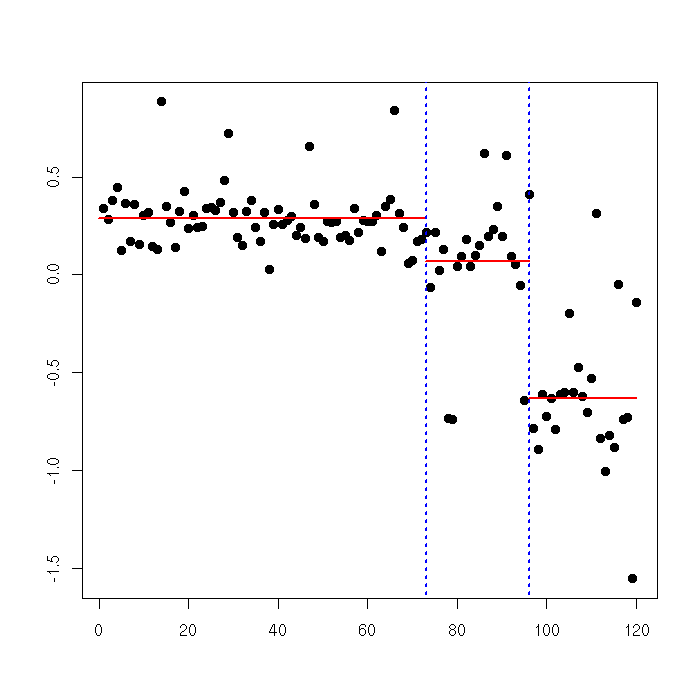
\includegraphics[width=4.5cm,
      height=2.5cm, clip=]{../Figures/CopyNumberChr10_BIC}  
    \end{tabular}
    &
    \begin{tabular}{l}
      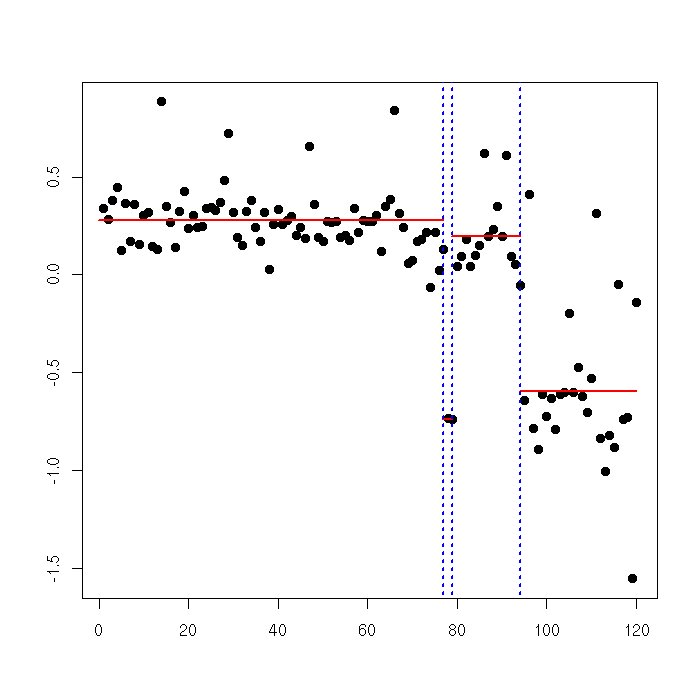
\includegraphics[width=4.5cm,
      height=2.5cm, clip=]{../Figures/CopyNumberChr10_ICL} 
    \end{tabular} \\ 
    \begin{tabular}{p{1.75cm}} Breakpoint position \end{tabular}
    &
    \begin{tabular}{l}
      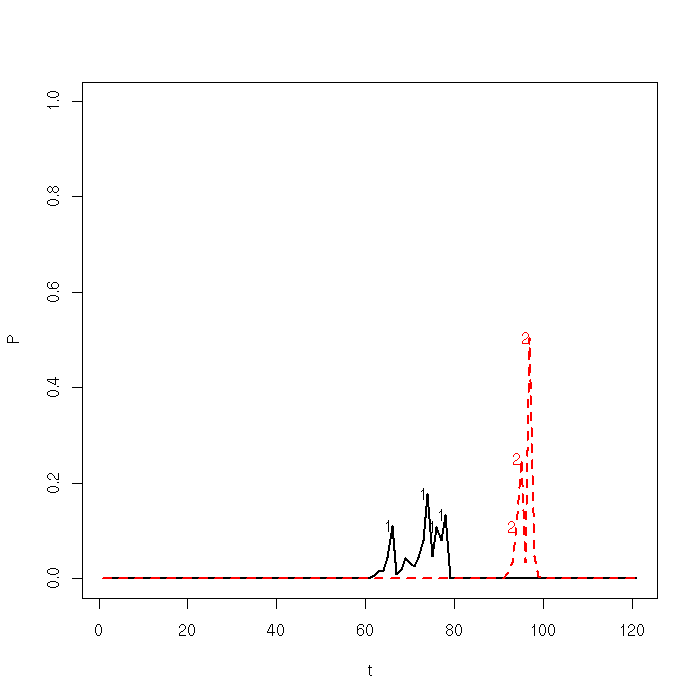
\includegraphics[width=4.5cm,
      height=2.5cm, clip=]{../Figures/CopyNumberChr10_ProbaBIC}  
    \end{tabular}
    &
    \begin{tabular}{l}
      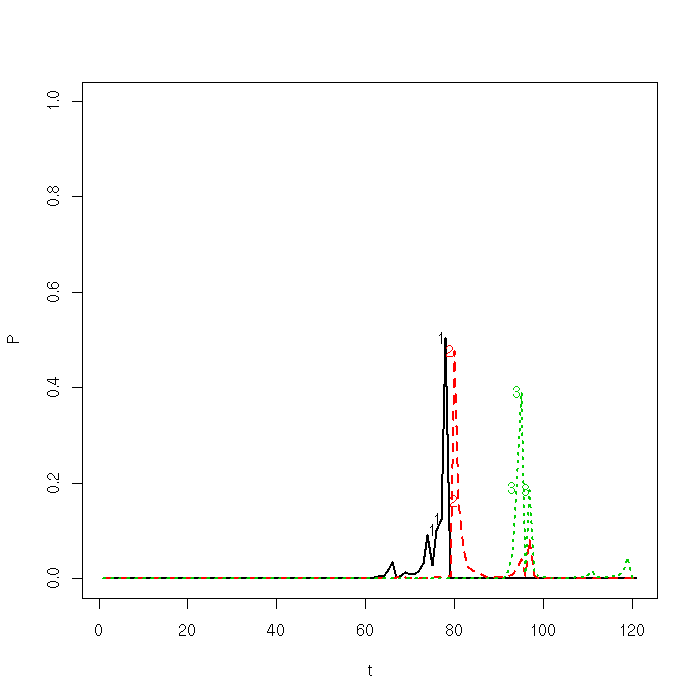
\includegraphics[width=4.5cm,
      height=2.5cm, clip=]{../Figures/CopyNumberChr10_ProbaICL} 
    \end{tabular} \\ 
    \begin{tabular}{p{1.75cm}} Segment probability \end{tabular}
    &
    \begin{tabular}{l}
      \vspace{-.5cm}
      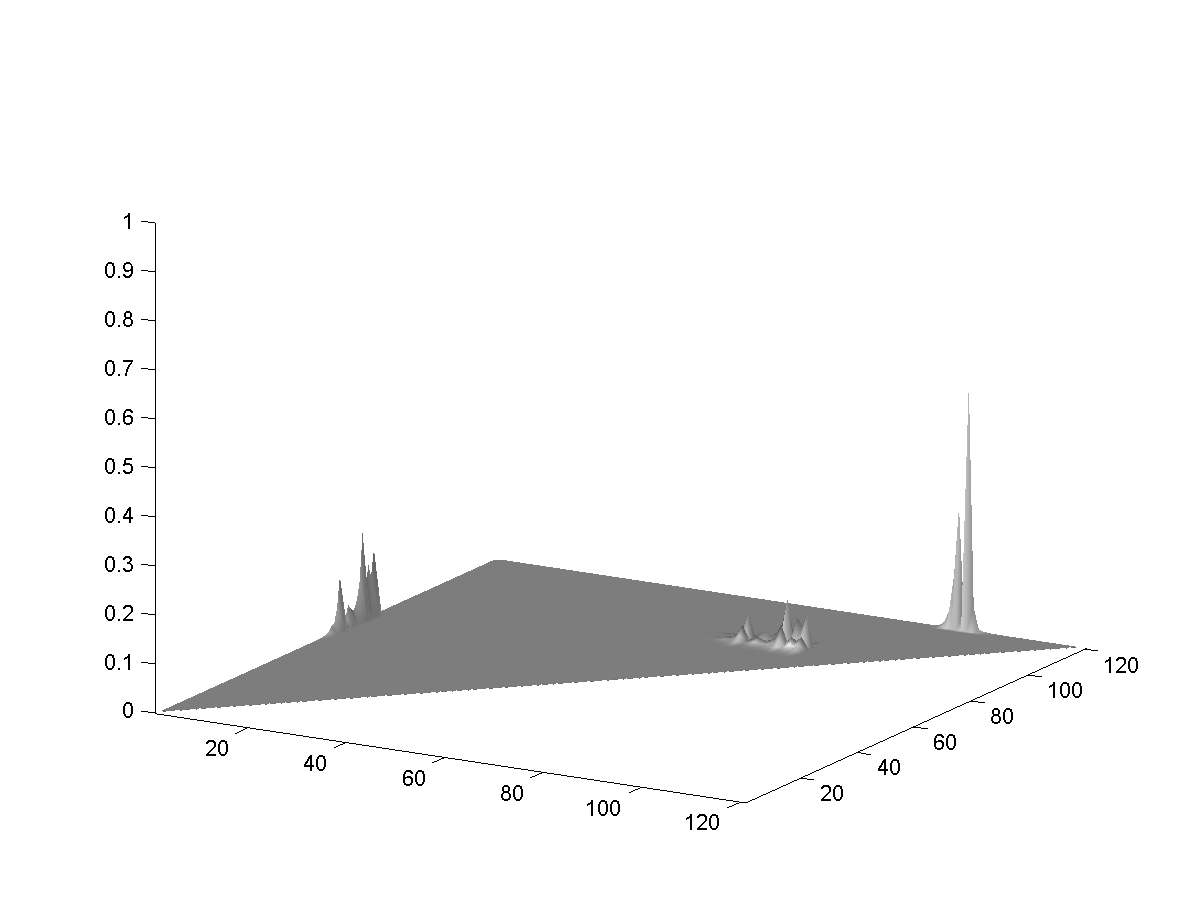
\includegraphics[width=4.5cm,
      height=2.5cm, clip=]{../Figures/ProbSeg-BIC}    
    \end{tabular}
    &
    \begin{tabular}{l}
      \vspace{-.5cm}
      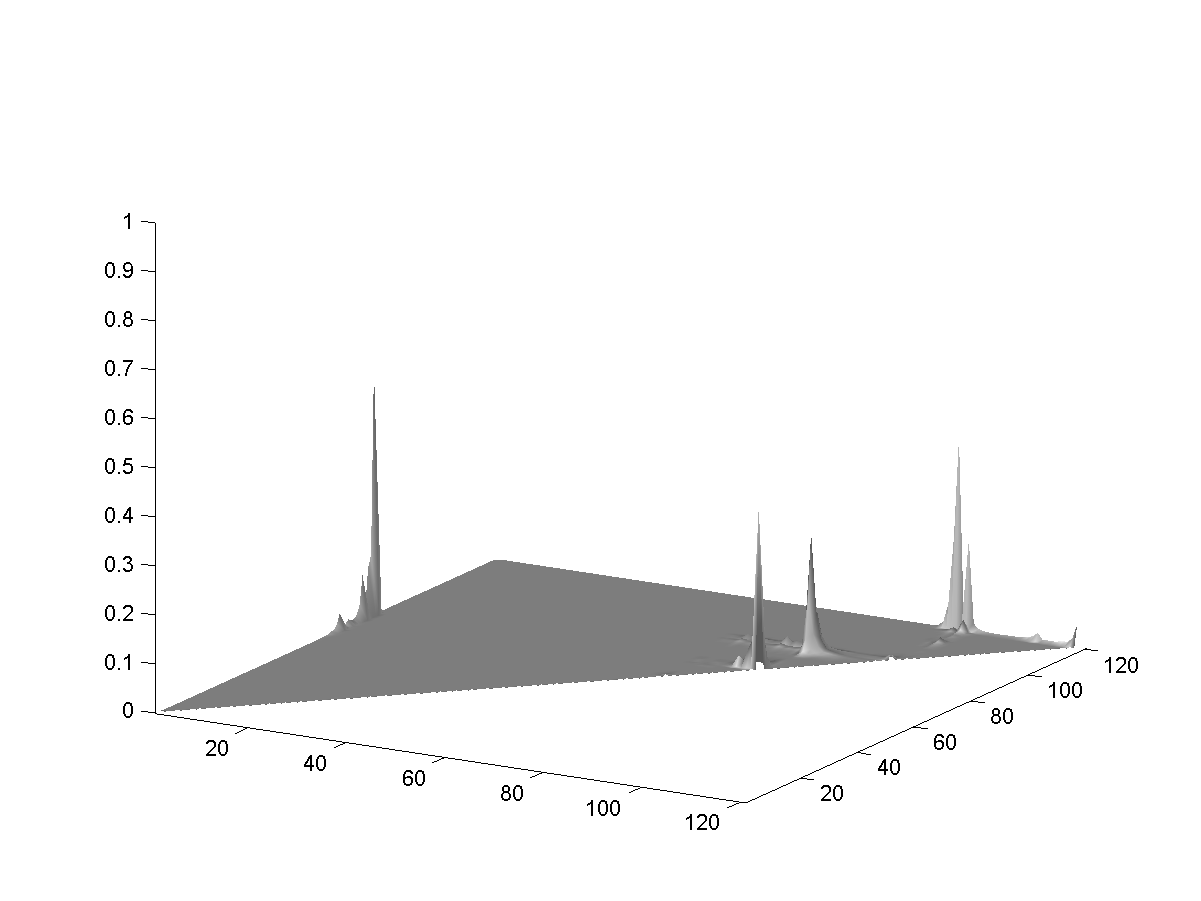
\includegraphics[width=4.5cm, height=2.5cm,
      clip=]{../Figures/ProbSeg-ICL}  
    \end{tabular} \\
  \end{tabular}
  $$
  }

%====================================================================
\subsection{Model selection}
\frame{ \frametitle{Choice of $K$: Penalised contrast}
%==================================================================== 
  \emphase{2-step strategy.} 
  \begin{enumerate}
  \item Best segmentation with dimension $K$
    $$
    \widehat{m}(K) = \arg\min_{m \in \Mcal_K} \ell(\Ybf, m)
    $$
  \item Best dimension $K$
    $$
    \widehat{K} = \arg\min_{K} \ell(\Ybf, \widehat{m}(K)) + \pen(K)
    $$
  \end{enumerate}
  \refer{Leb05}: 
  $$\pen(K) = f(|\Mcal_K|);$$
  \refer{Lav05}: 
  $$\pen(K) = \beta K.$$
  \begin{itemize} 
  \item \emphase{Constant penalty} within each dimension $\Mcal_K$.
  \item The best model \emphase{$\widehat{m}(K)$ does not depend} on
    the penalty $\pen(K)$.
  \end{itemize}
  }

%====================================================================
\frame{ \frametitle{Bayesian Information Criterion (BIC)}
%==================================================================== 
  Bayesian framework: \emphase{$\BIC(M) \approx \log p(M | \Ybf)$},
  based on the Laplace approximation:
  $$
  \log \int p(M, \theta | \Ybf) \dd \theta \approx \log p(M | \Ybf, \widehat{\theta})
  - \frac{\log n}2 \dim(M)
  $$
  \emphase{Segmentation context:  $\BIC(K)$}
  $$
  \Mcal_K = \bigcup_{m\ \in \Mcal_K} \text{span}(m)
  $$
  \begin{itemize}
  \item Regularity conditions \emphase{not fulfilled} when 'model' $M$
    $=$ dimension $K$.
  \item \refer{ZhS07}: \emphase{modified approximation}
    $$
    \pen(K) = f(|\Mcal_K|) + g\left(\emphase{\sum_{r \in \widehat{m}(K)}
        \log n_r}\right)
    $$
  \end{itemize}
  }

%====================================================================
\frame{ \frametitle{Exact BIC criteria}
%==================================================================== 
  \emphase{Choice of $K$.}
  $$
  \BIC(K) = \log p(\Ybf, K) = \log \left[\emphase{\sum_{m \in
        \Mcal_K}} p(m) \int p(\Ybf | m, \theta) p(\theta |m) \dd
    \theta \right].
  $$
  \emphase{Choice of $m$.}
  $$
  \BIC(m) = \log p(\Ybf, m) = \log \left[p(m) \int p(\Ybf | m,
    \theta) p(\theta |m) \dd \theta \right]
  $$
  where $p(m)$ must be normalised so that
  $$
  \sum_K \emphase{\sum_{m \in \Mcal_K}} p(m) = 1.
  $$
  }

%====================================================================
\frame{ \frametitle{ICL criterion}
%==================================================================== 
  \emphase{Incomplete data model context} (mixture model):
  \begin{itemize}
  \item \refer{BCG00} add an entropy term $\Hcal(K)$ to the $\BIC(K)$
    penalty
  \item $\Hcal(K)$ accounts for the reliability of the prediction of
    the unknown variable.
  \end{itemize}
  \bigskip 
  \emphase{Segmentation context.}
  \begin{itemize}
  \item Change-point positions can be view as unknown variables.
  \item For a given dimension $K$, it is desirable that the best
    segmentation clearly outperforms the others:
    $$
    \text{for any } m \in \Mcal_K \setminus \{\widehat{m}(K)\}:
    \quad p(\widehat{m}(K)|\Ybf) \gg p(m | \Ybf).
    $$
  \item This can be measured by the posterior entropy $\Hcal(K)$
  \end{itemize}
  \bigskip
  \emphase{ICL criterion:}
  $$
  \ICL(K) = \log \sum_{m \in \Mcal_K} p(\Ybf, m) - \Hcal(K)
  $$
    }

%====================================================================
\frame{ \frametitle{Comparison BIC/ICL: Simulation study}
%==================================================================== 
  \begin{columns}
    \begin{column}{0.45\linewidth}
      \emphase{Simulations: } Poisson signal with alternating
      means $\lambda_0$ and $\lambda_1$, $n = 100$. \\
      \bigskip \emphase{Criterion} = \% of recovery of the true number
      of segments ($K =
      5$). \\
      \bigskip
      \begin{itemize}
      \item $\BIC(m)$ achieves (much) better performances than
        $\BIC(K)$
      \item $\ICL(K)$ outperforms both $\BIC(K)$ and $\BIC(m)$.
      \end{itemize}
    \end{column}
    
    \begin{column}{0.45\linewidth}
      \begin{tabular}{c}
        \textcolor{green}{$\BIC(K)$} \quad \textcolor{red}{$\BIC(m)$} \quad
        \textcolor{blue}{$\ICL(K)$} \\
        ~\\
        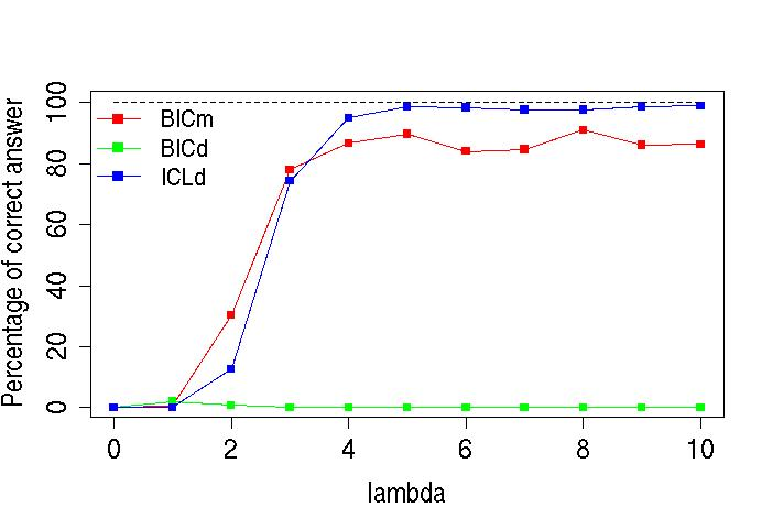
\epsfig{file=/Recherche/Ruptures/Exposes/Figures/ICLvsBIC.ps, clip=, bbllx=50, bblly=60,
          bburx=545, bbury=340, width=5cm, height=5cm} \\
        $\lambda_1 - \lambda_0$ ($\lambda_0 = 1$)
      \end{tabular}
    \end{column}
  \end{columns}
 }

%====================================================================
\frame{ \frametitle{}
%==================================================================== 
  \vspace{-1cm}
  $$
  \begin{tabular}{cc}
    \begin{tabular}{c}
      \emphase{\large Back to the example} \\
      \epsfig{file=/Recherche/Ruptures/Exposes/Figures/CopyNumberChr1_Alone.ps, 
        bbllx=38, bblly=40, bburx=565, bbury=385, width=4.25cm, height=2.25cm,
        clip=} \\
      \\
      $\BIC(K) \rightarrow \widehat{K} = 10$ \\
      \epsfig{file = /Recherche/Ruptures/Exposes/Figures/BIC2_NP.ps,
      width=5cm, height=2.5cm, clip=} \\
    \end{tabular}
    &
    \begin{tabular}{c}
%       \\
%       $\ICL(K) = f[\BIC(K)]$ \\
%       \epsfig{file=/Recherche/Ruptures/Exposes/Figures//BICandEntropy.ps,
%       clip=, scale=0.25, bbllx=38, bblly=40, bburx=565, bbury=385}    
      $\BIC(m) \rightarrow \widehat{K} = 3$ \\
      \epsfig{file = /Recherche/Ruptures/Exposes/Figures/BIC_NP.ps,
      width=5cm, height=2.5cm, clip=} \\
      \\
      $\ICL(K) \rightarrow \widehat{K} = 4$ \\
      \epsfig{file = /Recherche/Ruptures/Exposes/Figures/ICL_NP.ps,
      width=5cm, height=2.5cm, clip=} \\
    \end{tabular}
  \end{tabular}
  $$
  When $K$ exceeds the 'true' dimension, all segmentations
  nested within the 'true' one have a high posterior probability,
  which increases the entropy. 
}

%====================================================================
\frame{ \frametitle{Comments}
%====================================================================   
  \begin{itemize}
  \item \emphase{Exact computation} of BIC criteria can be achieved in
    $\Ocal(n^2)$.
  \item Either \emphase{the dimension $K$ or the segmentation $m$} can
    be selected.
  \item Based on simulations, \emphase{BIC penalties seem too weak}
    (although there computation is exact).
  \item Interestingly, in the Gaussian case when using conjugate
    priors (Normal / inverse Gamma), the exact computation of $\log
    p(m |\Ybf)$ gives raise to a term in
    $$
    \log \left(\prod_{r \in m} n_r\right)
    $$
    similar to the one of \refer{ZhS07}.
  \end{itemize}
  }

%====================================================================
\section{Conclusions}
\frame{ \frametitle{Some conclusions} 
%==================================================================== 
  \begin{itemize}
  \item It may be worthy to tackle combinatorial problems to still
    compute \emphase{exact quantities} (in place of stochastic or asymptotic
    approximations).
  \item Combinatorists (or computer scientists) can help statisticians
    to \emphase{identify problems that can actually be solved}.
  \end{itemize}

  \bigskip \pause
  \paragraph{Bio-molecular data} constitute a never ending source of
  such problems. 

  \bigskip
  \paragraph{Ex.: Network motifs} (triangles,
  cliques, loops, 'whiskers', etc.) play a role in network analysis
  similar to the one of oligonucleotides in DNA sequences analysis:
  \begin{itemize}
  \item Can we enumerate them in large graphs?
  \item What is the distribution of their count in non-naive random
    graph models?
  \item How does the motif topology influence all this?
  \end{itemize}
  }

% %====================================================================
% %====================================================================
% \section{Interaction networks and Motif counting}
% \frame{ \frametitle{Interaction networks and Motif counting}
% %====================================================================

%   }

% %====================================================================
% %====================================================================
% \subsection{Biological networks}
% \frame{ \frametitle{Biological networks}
% %====================================================================

%   }

% %====================================================================
% %====================================================================
% \subsection{Network motifs}
% \frame{ \frametitle{Network motifs}
% %====================================================================

%   }

%====================================================================
\frame{ \frametitle{References}
%==================================================================== 
  {\tiny
    \bibliography{/biblio/AST,/biblio/ARC}
    \bibliographystyle{/latex/astats}
    }
  }

%====================================================================
%====================================================================
\end{document}
%====================================================================
%====================================================================
